\label{sec:studyDesign}
In this sub-section, we describe the details of the data collection and processing approach followed to answer our different research questions.





\subsection{Data Collection}
\label{sec:dataCollection}
The development of the design smell detection system was based on code samples of deep learning programs. These examples represent deep learning programs in which design smells are introduced. These samples were collected by Nikanjam et al. \cite{nikanjam2021design} as part of their empirical study of design smells in deep learning programs. Indeed, in this study, they presented samples of deep learning programs containing the design smells listed in the introduction \ref{sec:codeSmell}. These source code examples were collected from the StackOverflow and Github platforms.\\\\

The designed smell detection system thus developed was used on a set of deep learning programs collected from the GitHub platform. These deep learning programs were collected according to a well-defined process. We used the GitHub API and, more precisely, search queries of the type \emph{search code}. This query searches Github repositories for files containing specific keywords defined in our system. As our paper focuses solely on the \emph{Keras}, \emph{Tensorflow} and \emph{Pytorch} frameworks, we have used the keywords presented in the table \ref{tab:keywords}. These keywords represent the modules and functions of these three frameworks.\\


\begin{table}[h]
  \centering
  \caption{\emph{List of keywords used to search for deep learning programs in Github repositories.}}
  \label{tab:keywords}
  \begin{tabular}{ll}
    \toprule
    \textbf{Key word}          & \textbf{Framework} \\ \midrule
    keras.layers               & Keras              \\
    keras.layers.convolutional & Keras              \\
    AveragePooling2D           & Keras/TensorFlow   \\
    MaxPooling2D               & Keras/TensorFlow   \\
    tensorflow.keras.layers    & Tensorflow         \\
    Conv2D                     & Keras/TensorFlow   \\
    Convolution2D              & Keras/TensorFlow   \\
    BatchNormalization         & Keras/TensorFlow   \\
    import torch               & Pytorch            \\
    import torchvision.models  & Pytorch            \\
    torch.nn.Sequential        & Pytorch            \\
    torch.nn.Conv2d            & Pytorch            \\
    torch.nn.BatchNorm2d       & Pytorch            \\
    torch.nn.MaxPool2d         & Pytorch            \\ \bottomrule
  \end{tabular}
\end{table}


The search query type \emph{search code} returns a set of information about the
repository and the file containing the searched keywords. This returns a raw
data set of 9572 different Github repositories. We then randomly select a subset
of 10\% of our raw data set, i.e. 958 Github repositories, in order to optimize
the manual filtering step below. From this subset, we then filter the
directories according to the following criteria:
(1) the number of commits ($\geq$ 100), (2) the number of stars ($\geq$ 100),
(3) last commit date ($\leq$ 5 years), (4) the number of contributors ($\geq$
5). This filtering allows us to keep only the most popular and active
directories. We then filtered the directories manually, eliminating projects
that are not deep learning programs or not relevant to our study (don't use the
chosen frameworks, or don't implement neural networks). As a result, we ended up
with 500 projects on which to apply our design smell detection system. \\The
schema \ref{fig:data_collect} presents the process of collecting deep learning
programs.\\

\begin{figure*}[h]
  \centering
  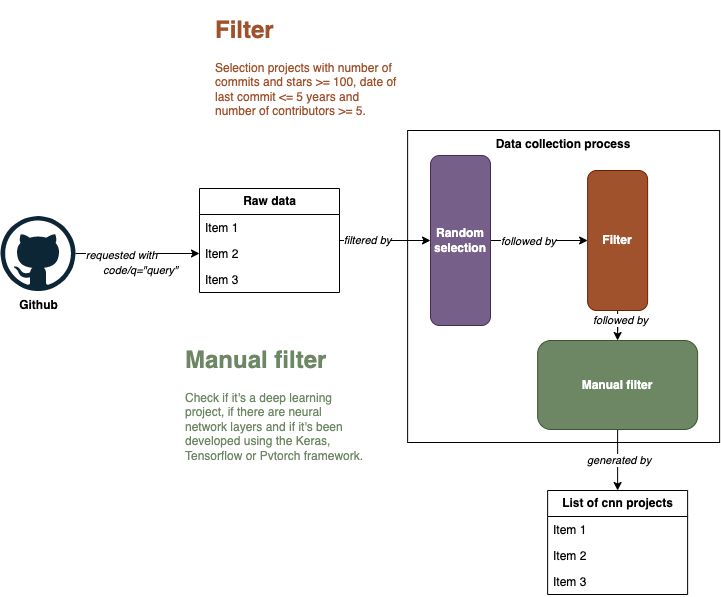
\includegraphics[width=0.8\textwidth]{figure/design_smell_data_collection.png}
  \caption{\emph{Process for collecting deep learning projects in Github.}}
  \label{fig:data_collect}
\end{figure*}






\subsection{Data Processing}
\label{sec:DataProcessing}
The process of collecting deep learning programs has provided us with a set of deep learning programs on which we will apply our design smell detection system. However, it's important to note that the deep learning programs in our case are programs written solely in the Python language. It is therefore essential to note that, the design smell detection system developed in this paper is a system that is only capable of detecting design smells in deep learning programs written in the Python language.\\

In order to answer the research question \emph{RQ1}, we have developed a system for detecting design smells in deep learning programs. This system is divided into three parts. The first part deals with the modeling of deep learning programs. The second part concerns the detection of design smells in deep learning programs. The third is the analysis of detection results.\\

\subsubsection{Modeling deep learning programs}
\label{sec:modelingDeepLearningPrograms}
Modeling deep learning programs is the first step in the design smell detection process. This involves transforming the source code of the collected deep learning programs into an intermediate model that will be used for design smell detection. This intermediate model is a \emph{Famix Abstract Syntax Tree} (\emph{FAST}) model \ref{fig:fast}. The \emph{FAST} model is used to represent programs as syntax trees. It inherits from the abstract source code representation \emph{Famix} developed in the \emph{Pharo} programming language. With \emph{Famix}, source code is represented in object form and according to a defined metamodel to symplify the analysis and representation of complex programs. A \emph{Famix} model is a language-agnostic representation of the original source code and includes functions for navigation and transformation.\\

\begin{figure*}[h]
  \centering
  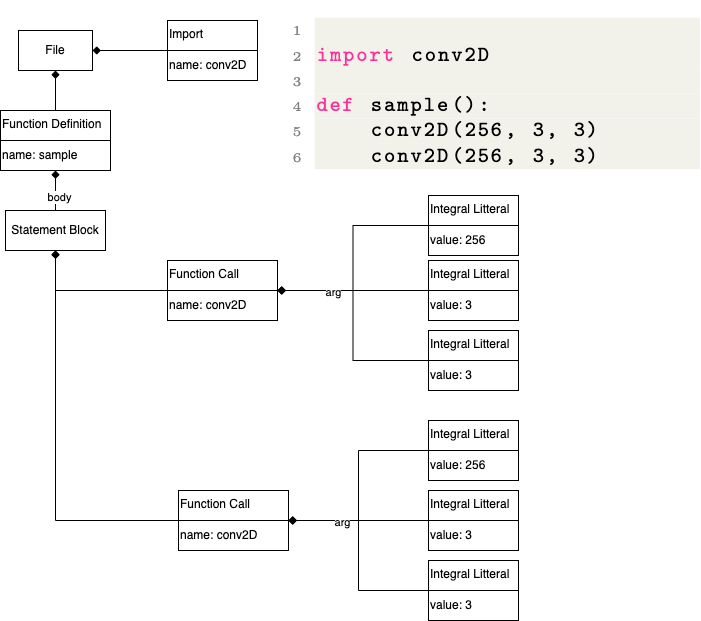
\includegraphics[width=0.8\textwidth]{figure/fast.png}
  \caption{\emph{Sample \emph{FAST} model of a fictive deep learning program.}}
  \label{fig:fast}
\end{figure*}

Transformation of the collected source code into the \emph{FAST} model is as follows. Each collected project is cloned into a local directory. Its source code is then parsed using the Python library \emph{ast.py}. This library transforms the source code into a syntax tree in \emph{json} form. The resulting \emph{json} is then transformed into a \emph{FAST} model using an importer developed under the visitor design pattern. Visitors are functions that can navigate a syntax tree to perform specific operations on its nodes. In our case, we have developed visitors that enable us to browse the syntax tree (\emph{json}) and transform each node of this tree into a \emph{FAST} entity.\\

The diagram \ref{fig:modelling} illustrates the modeling process for deep learning programs.\\

\begin{figure*}[h!]
  \centering
  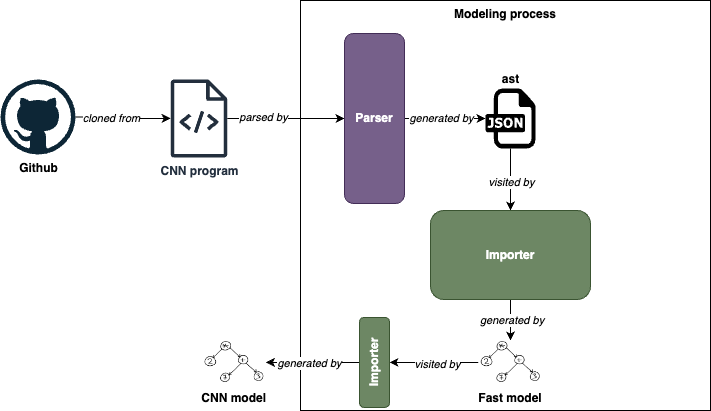
\includegraphics[width=0.8\textwidth]{figure/design_smell_modeling.png}
  \caption{\emph{Modeling process for deep learning projects.}}
  \label{fig:modelling}
\end{figure*}


\subsubsection{Design smell detection}
\label{sec:designSmellDetection}
The \emph{FAST} model obtained from the modeling of deep learning programs is then used for design smell detection. This step consists of browsing the \emph{FAST} model and applying design smell detection rules. These rules are defined in the \emph{Pharo} programming language. One or more rules can be applied to a node in the syntax tree to detect a design smell.\\

% Le schema \ref{fig:rules} est un exemple de règle
% permettant de détecter l'odeur de conception numéro 5 - \emph{Non-dominating down-sampling}.\\
The diagram \ref{fig:detection} illustrates the design smell detection process.\\


\begin{figure*}[h!]
  \centering
  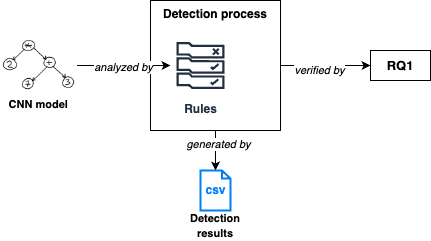
\includegraphics[width=0.8\textwidth]{figure/design_smell_detection.png}
  \caption{\emph{Design smell detection process.}}
  \label{fig:detection}
\end{figure*}

\subsubsection{Analysis of design smell detection results}
\label{sec:AnalysisOfDesignSmellDetectionResults}
The results of each repository's design smell detection are stored in the form \emph{csv}. For each repository, we record the name of each design smell detected, the number of times that smell is detected in a repository file and the path to that file. These results are used to answer the research questions \emph{RQ2} and \emph{RQ3}.\\
We then calculate the distribution of design smells in each repository by dividing the number of occurrences of a design smell by the total number of design smells detected in the repository. This distribution answers the research question \emph{RQ2}. The distribution of design smells across all 500 repositories is also calculated by dividing the number of occurrences of a design smell by the total number of design smells detected across all 500 repositories. This distribution also answers the research question \emph{RQ2}.\\

We then calculate the correlation matrix between design smells in all 500
repositories. This matrix answers the research question \emph{RQ3}. A
correlation matrix is used to calculate the correlation between two variables.


A correlation coefficient is calculated using the following formula:  $r =
  \frac{cov(X,Y)}{\sigma_X \sigma_Y}$  where $r$ is the correlation coefficient, $cov(X,Y)$ is the covariance between the two variables $X$ and $Y$, $\sigma_X$ is the standard deviation of the variable $X$ and $\sigma_Y$ is the standard deviation of the variable $Y$. This correlation coefficient ranges from -1 to 1. A positive correlation exists when the correlation coefficient ranges from 0 to 1. In this case, the closer it is to 1, the more positively correlated the two variables are, and the closer it is to 0, the less correlated the two variables are. A negative correlation is defined as a correlation coefficient between -1 and 0. In this case, the closer the correlation coefficient is to -1, the more negatively correlated the two variables are, and the closer it is to 0, the less correlated the two variables are.\\



In our case, the variables are the design smells. The correlation between two design smells is calculated by dividing the number of occurrences the two design smells are detected together by the total number of times the two design smells are detected. This correlation is calculated for each pair of design smells. The closer it is to 1, the more the two design smells are correlated, and the closer it is to 0, the less the two design smells are correlated.\\

A positive correlation means that the two design smells are often detected together. A negative correlation means that the two design smells are rarely detected together. Finally, a zero correlation means that the two design smells are never detected together.\\

The diagram \ref{fig:analysis} illustrates the process of this last part.\\

\begin{figure*}[h!]
  \centering
  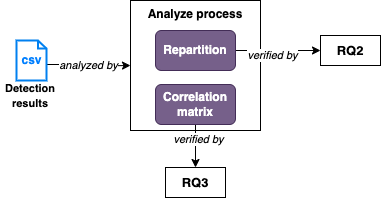
\includegraphics[width=0.8\textwidth]{figure/design_smell_analyze.png}
  \caption{\emph{Process for analyzing design smell detection results.}}
  \label{fig:analysis}
\end{figure*}

\subsection{Replication Package}
\label{sec:Replication Package}
Source code for the \emph{json} syntax tree source code parser is available on Github at \url{https://github.com/aurpur/parserPythonToJson}, and source code for the smell detection system is available on Github at \url{https://github.com/aurpur/famixPythonImporter}. The data collection system is also available on Github at \url{https://github.com/aurpur/ms-github-data-collection}.\\
